\setlength{\footskip}{8mm}

\chapter{LITERATURE REVIEW}


\begin{figure}
    \caption{Raman spectra of glucose solution at different concentration \citep{solutionGlucose}.}
    \centerline{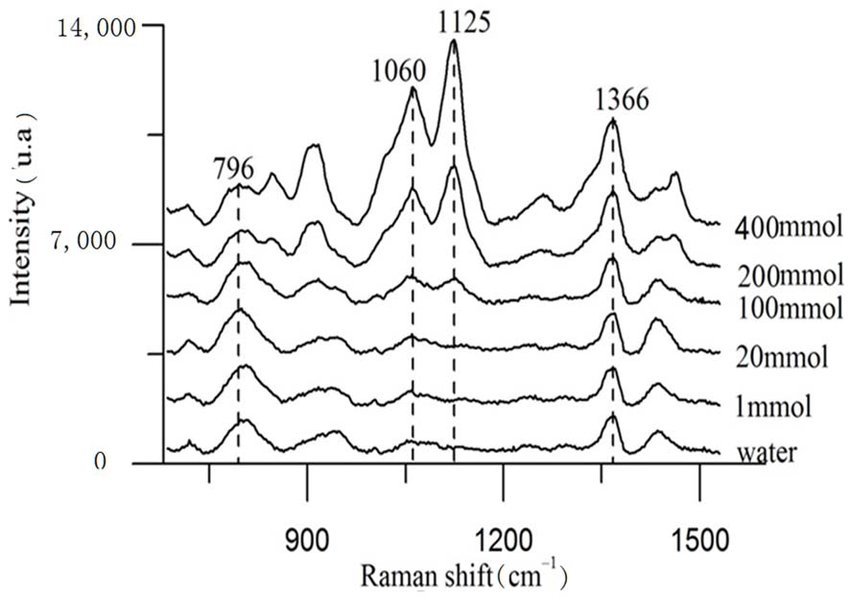
\includegraphics[width=3in]{figures/solutionGlucose-RS.jpeg}} \label{fig:solutionGlucose-RS}
    % \small{\textit{Note.} Additional notes goes here.}
\end{figure}

\begin{figure}
    \caption{A trace of glucose fingerprint in Raman scattering of in vivo blood \citep{solutionGlucose}.}
    \centerline{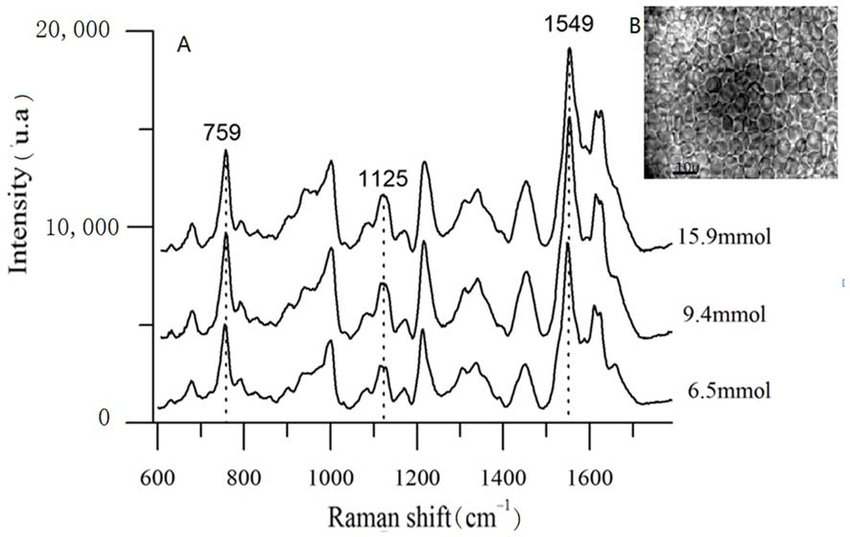
\includegraphics[width=3in]{figures/bloodGlucose-RS-2012.jpeg}}\label{fig:bloodGlucose-relative1125}
    % \small{\textit{Note.} Additional notes goes here.}
\end{figure}

The Raman spectra of amorphous glucose (glucose fingerprint) when in combination with water (glucose solution) and blood (blood glucose) are examined. Following that, we will look at measurement sites, preprocessing strategies, and data modeling.
\\
\section{Glucose Fingerprint}
When glucose has been included in the analyte, the "glucose fingerprint" shows as a distinctive Raman scattering spectrum. 
Peaks in Raman scattering in glucose solution (glucose and water) are 796, 1060, 1125, and 1366 $cm^-1$ respectively (Figure~\ref{fig:solutionGlucose-RS}). These peaks rise as glucose concentration rises, demonstrating a quantitative characteristic of Raman spectroscopy (Shao et al., 2012).
When measuring Raman scattering of ISF, the glucose fingerprint is also visible in a more complex analyte such as blood. (González Viveros et al., 2022; Kang et al., 2020; Scholtes-Timmerman et al., 2014) as show in Figure 2.4. Kang et al. (2020) extract the glucose fingerprint, which contains a peak at 1125 $cm^-1$, from two noisy Raman signals. As a result, Raman spectroscopy can identify blood glucose.

\begin{table}[]
\caption{Assignments of Raman peaks that are identified in the spectra of the microvessels and blood \citep{peak45,forearm2005,peak47,peak48}}
\begin{center}
\begin{tabular}{cccc}
\hline
\multicolumn{2}{l}{Peak Position ($\text{cm}^{-1}$)} & \multirow{2}{*}{Assignments}  & \multirow{2}{*}{Components} \\ \cline{1-2}
Microvessels         & Blood         &                               &                             \\ \cline{1-2}
\hline
650                  & 643           & P:C-S str                     & Ascorbic acid               \\
758                  & 752           & $\nu_{15}$                    & Trp                         \\
837                  & 827           & $\gamma10$                    & Fructose                    \\
858                  & 855           & $\nu(C-C)$                    & Tyr, lac                    \\
885                  & -             & -                             & -                           \\
902                  & 898           & p:C-C skeletal                & Tyr                         \\
945                  & 940           & $\nu(C-C)$                    & Crtic acid                  \\
978                  & 971           & p: Skeletal vibr              & Fibrin                      \\
1004                 & 1004          & $\nu$-ring                    & Phe                         \\
1027                 & 1026          & $\delta(={C}_{b}{H}_{2})$asym & Lac                         \\
1130                 & 1129          & $\nu_5$,                      & Lac                         \\
1163                 & 1157          & $\nu_{44}$                    & Heme                        \\
1217                 & 1212          & $\nu_5 + \nu_{18}$            & Heme                        \\
1320                 & 1321          & p: CH2 twist                  & Try                         \\
1332                 & 1341          & $\nu_{41}$                    & Trp                         \\
1424                 & 1423          & $\nu_{28}$                    & Acetates                    \\
1448                 & 1450          & $\delta(={CH}_{2}/{CH}_{3})$  & Trp                         \\
1551                 & 1546          & $\nu_{11}$                    & Heme                        \\
1608                 & 1603          & $\nu(C=C)_{\text{venyl}}$     & Heme                        \\
1660                 & 1653          & Amide I                       & Heme                        \\
\hline
\end{tabular}
\label{tab:bloodpeak}
\end{center}
\end{table}


\section{Measuring sites}
According to the thickness of human skin changes from place to place, Raman scattering measurements done at different locations may yield different findings (González Viveros et al., 2022; Li et al., 2019). If the laser is focused on the blood vessels, the glucose fingerprint signal will be greater (Shao et al., 2012). The stratum corneum (SC), epidermis, and dermis are the three layers of human skin (Li et al., 2019). When detecting glucose in ISF rather than blood, the following issues may arise: (1) ISF glucose lags after blood glucose (Cengiz \&\ Tamborlane, 2009; Steil et al., 2005), and (2) the concentration of glucose in ISF is much lower than blood (O'Kane, 2012). From the foregoing, the signal from glucose Raman scattering is weak (Li et al., 2019). Considering a better technique, it would be to measure the Raman signal in locations where the laser can better penetrate the dermis, because the dermis contains microvessels (Cutolo, Grassi, \&\ Matucci Cerinic, 2003; Ingegnoli, Smith, Sulli, \&\ Cutolo, 2018).
\cite{ramanNailFold2019} finds the greater $R^2 = 0.98$ prediction correlation when nailfold is used as a measuring site.
The result is better than the forearm ($R^2 = 0.83$) \citep{forearm2005,forearm2014} and fingertip ($R^2 = 0.91$) \citep{fingertip2011}.
\cite{sitecompare} measures Raman glucose at forearm, wrist, and index fingertip and achieves the root-mean-square error (RMSE) of $56.31\pm4.28$, $58.22\pm1.03$, and $56.65\pm8.99$ ml/dL respectively.

\section{Preprocessing techniques and Data modeling}

\begin{figure}
    \caption{(\textbf{A}) Blood glucose value with 1125 $\text{cm}^{-1}$ relative intensity. (\textbf{B}) Concentration-dependent Raman relative intensities of glucose (1125 $\text{cm}^{-1}$) \citep{solutionGlucose}}
    \centerline{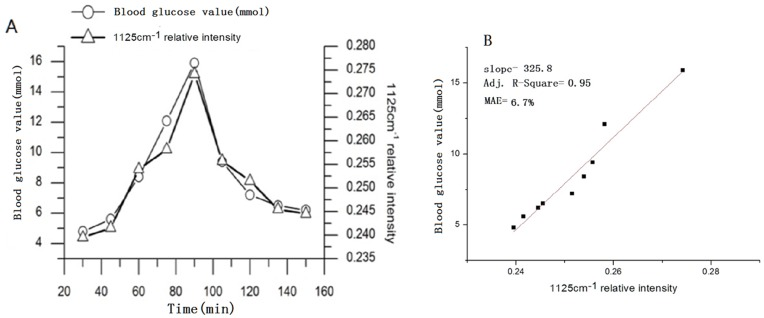
\includegraphics[width=3in]{figures/bloodGlucose-relative1125.png}}\label{fig:bloodGlucose-relative1125}
    % \small{\textit{Note.} Additional notes goes here.}
\end{figure}

\begin{figure}
    \caption{(\textbf{B}) Showing the linear relationship between normalized 1125 $\text{cm}^{-1}$ with blood glucose ($R^2 = 0.94$) \citep{directGlucose}}
    \centerline{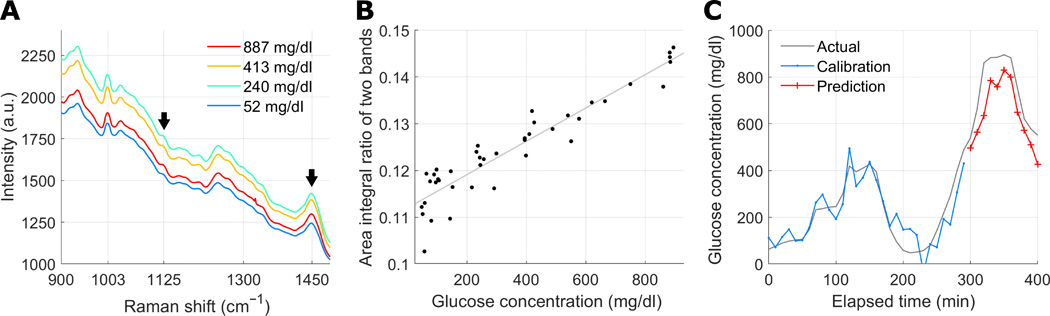
\includegraphics[width=3in]{figures/bloodGlucose-relative1125-directGlucose.jpeg}}\label{fig:bloodGlucose-relative1125-directGlucose}
    % \small{\textit{Note.} Additional notes goes here.}
\end{figure}

Preprocessing is largely divided into two categories. 
Using either the extracted features or the whole Raman spectrum as an input.
The complete spectrum analysis with partial least squares (PLS) is a popular method. \citep{forearm2014, sitecompare, forearm2005, directGlucose}.
The results vary from $R^2 = 0.62$ \citep{directGlucose}, $R^2 = 0.83$ \citep{forearm2005,forearm2014}, and RMSE of around 65 $\pm$ 0.4 ml/dL in~\cite{sitecompare}.
The preprocessing can be done by hand-pick \citep{directGlucose,solutionGlucose} or automatically \citep{ramanNailFold2019, sitecompare} pick the features.
Hand-pick features were performed by normalizing the spectra with either protein and lipid peaks (1450 $\text{cm}^{-1}$) \citep{directGlucose} or hemoglobin peaks (1549 $\text{cm}^{-1}$) \citep{solutionGlucose}.
It is demonstrated that the normalized 1125 $\text{cm}^{-1}$ has a linear correlation with in vivo blood glucose at $R^2 = 0.95$ \citep{solutionGlucose}.
In~\cite{directGlucose}, normalized 911, 1060, 1125 $\text{cm}^{-1}$ with 1450 $\text{cm}^{-1}$ were utilized as inputs of the more complex multiple linear regression (MLR) which achieved $R^2 = 0.91$.